\documentclass[11pt,oneside, final]{fithesis2}  
\usepackage[english]{babel} % package for multilingual support  
\usepackage[utf8]{inputenc} % Windows OS encoding  
\usepackage[T1]{fontenc}  
\usepackage{lmodern}
\usepackage{cmap}

\usepackage[plainpages=false,pdfpagelabels,unicode]{hyperref}
\usepackage[numbers, sort]{natbib}
\usepackage{graphicx}
\usepackage{multirow}
\usepackage{siunitx}

%\usepackage[linenumbers,noindent]{stdpage} %1800 character standard pages

%\renewcommand{\baselinestretch}{1.2}	% 1.2 radkovani
 
\thesistitle{Engine for drawing isometric game graphics in SVG} % enter thesis title  
\thesissubtitle{Master's thesis}  
\thesisstudent{Bc. Vít Svoboda}    % name of the author  
\thesiswoman{false}          % defines author?s gender  
\thesisfaculty{fi}  
\thesisyear{spring 2015}  
\thesisadvisor{Mgr. Marek Grác, Ph.D.} % fill in advisor?s name  
\thesislang{en}                 % thesis is in English  
 
\begin{document}  
\FrontMatter  
\ThesisTitlePage  
 
\begin{ThesisDeclaration}  
\DeclarationText  
\AdvisorName  
\end{ThesisDeclaration}  
 
\begin{ThesisThanks}  
I would like to thank my advisor for patience and academic guidance. I would also like to thank Ing. Ondřej Žižka for technical guidance.
\end{ThesisThanks}  
 
\begin{ThesisAbstract}  

\end{ThesisAbstract}  
 
\begin{ThesisKeyWords}  
5-10 key words, one key word can be multiple words. Key words are comma separated. Not the list of used technologies!
\end{ThesisKeyWords}  
 
\MainMatter
 
\tableofcontents          % prints table of contents  
 
\chapter{Introduction}
Browser games used to be built using the flash\cite{}. Specification of HTML5 introduced two new elements to display graphics: canvas and svg\cite{w3_html5}. With the broad adoption of the standard the focus shifted to the canvas element\cite{}. Is it possible to utilize other new element the same way? Chapter \ref{theory} briefly describes the current state of graphics engine usage and expectations. Furthermore this chapter elaborates on the specifics of web graphics. Chapter \ref{solution} describes the suggested alternative and Chapter \ref{tech} summarizes technologies used in the attempted implementation. The actual implementation is described in Chapter \ref{implementation} and subjected to criticism in Chapter \ref{testing}.

\chapter{State of the art}
\label{theory}

\section{What is a graphic engine}
Graphic engine\footnote{Sometimes also called rendering engine\cite{}} is a software component responsible for transforming a logical model of a scene to an image on the screen. In video games this is usually a part of game engine also responsible for collision detection, physics calculation, game logic script execution\cite{}. Graphic engines used in native applications heavily depend on middleware like OpenGL or DirectX\cite{}. 

\subsection{Typical functionality provided by an engine}
The input for a graphic engine is a set of objects on the scene, data representing their appearance (sprites, meshes and textures) and a camera position. Engine has to determine what objects or their parts are currently visible from the point of view of the given camera and either prepare a bitmap in memory containing graphic representation of all related objects. Usually the last part is done via calls of some underlying API rather than manipulating the bitmap directly. Optionally the engine can perform various post-processing on the output, such as anti-aliasing, shading etc. More complex post-processing is usually performed only in 3D applications. When rendering a real-time image, the process has to be repeated several times per second to maintain perception of a fluid animation. Simply put, the higher frame rate\footnote{Frame rate is often referred to as FPS (Frames Per Second) with values in Hz.}, the better\cite{claypool}. Nowadays the frame rate is limited by standard display hardware with 60Hz refresh rate, but new hardware allowing to display image on 120, 144 Hz or ever more is emerging on the market.

\section{Isometric graphics}
Isometric projection is an axonometric projection\footnote{Projection of an object rotated along one or more axes relative to the plane of projection\cite{}.} with perpendicular direction of the projection and equal angle between the vew plane and all axes\cite{desai} as shown in Figure \ref{isometric}. This way all 3 dimensions can be displayed sufficiently enough to allow orientation while keeping the rendering simple and therefore fast. 

\begin{figure}[htp]
	\centering
	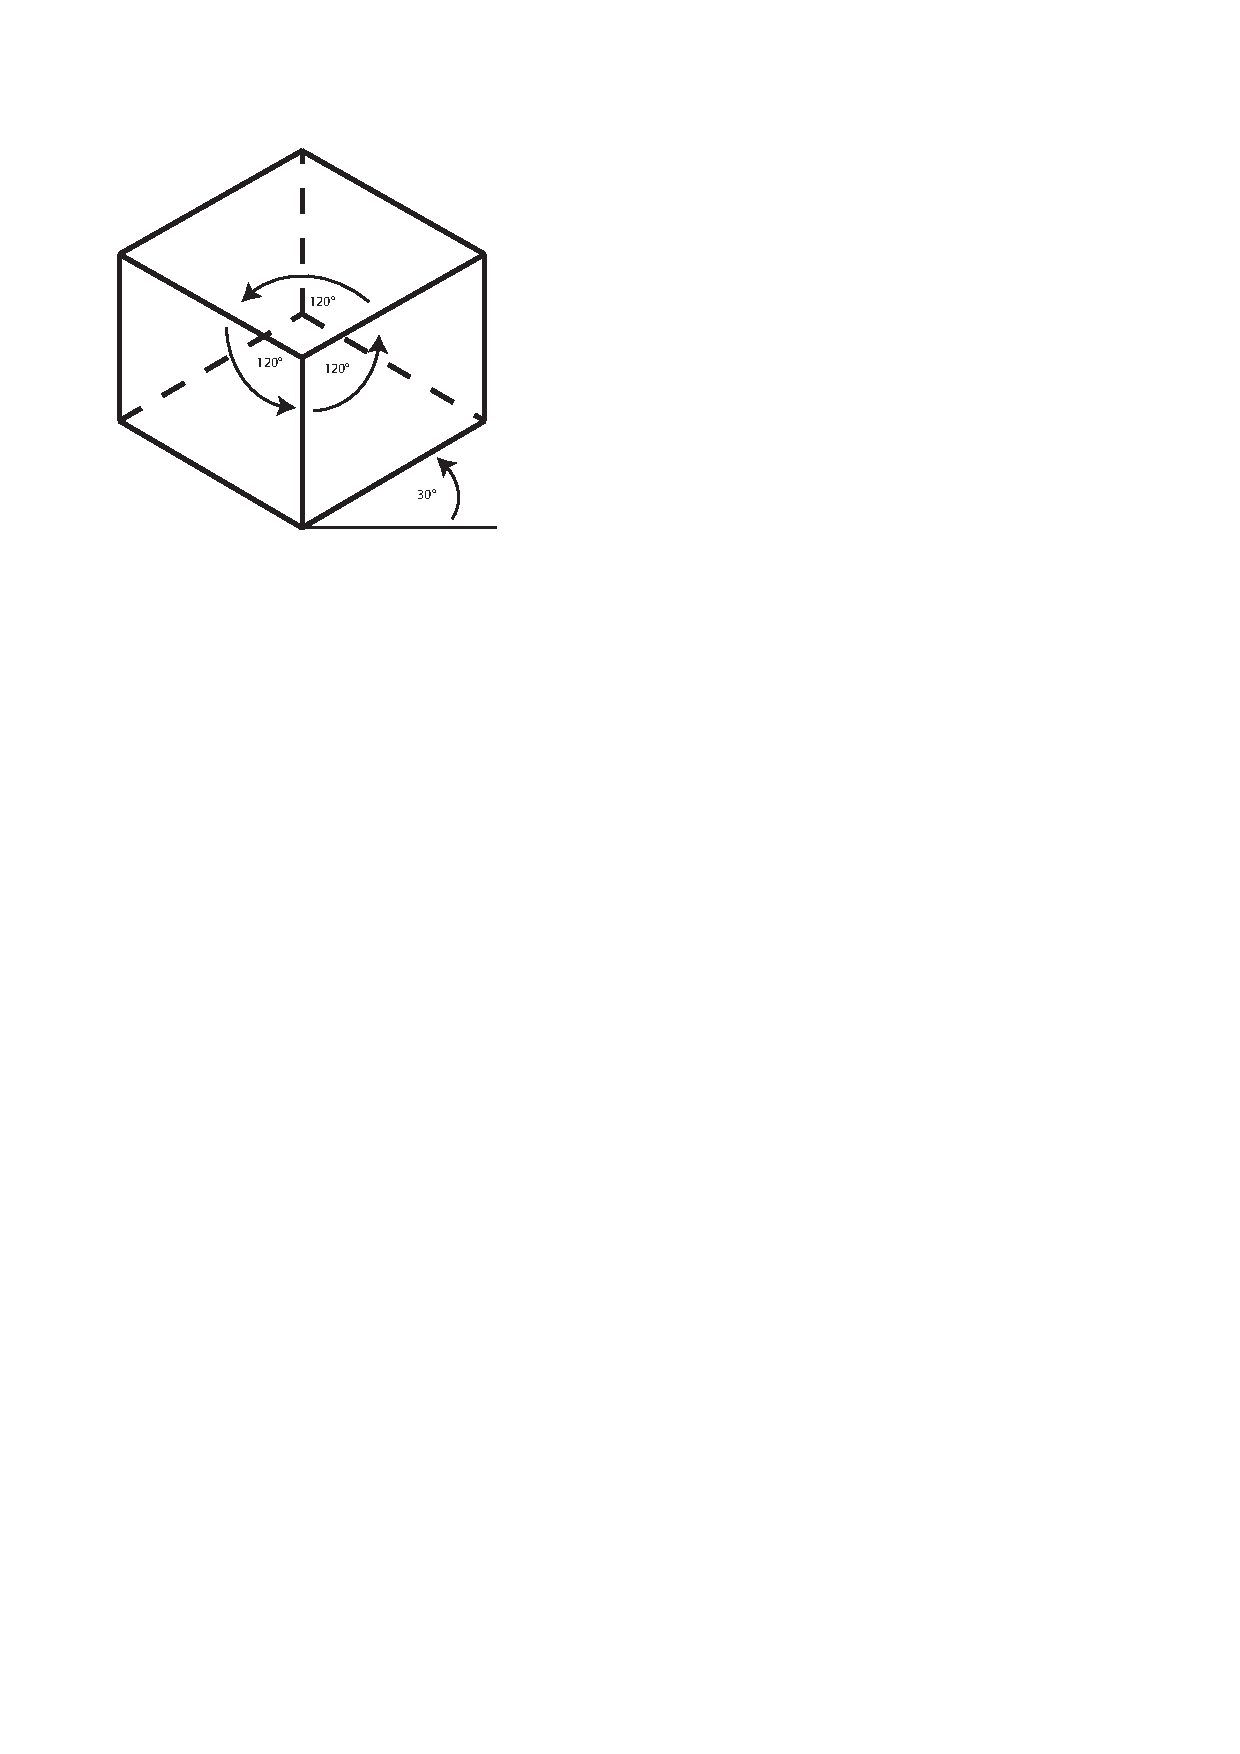
\includegraphics[clip=true,trim=0 205mm 100mm 0]{thesis-isobox}
	\caption{Isometric projection}
	\label{isometric}
\end{figure}

\subsection{Isometric camera}
The camera is top down, but tilted by 45 degrees in both directions. The diagonals therefore should be at 30 degrees, but due to the irregular aliasing of these diagonals on the bitmap grid the practical approach is slightly different. The image is rotated by 45 degrees and then the aspect ratio is changed to 2:1. The result are regular 2pixel stairs forming diagonals in about 26.565 degrees\footnote{\begin{math}\arctan \frac{1}{2} \approx 26.565\si{\degree}\end{math}}. This eliminates trigonometry from the projection mathematics allowing faster rendering.

\begin{figure}[htp]
	\centering
	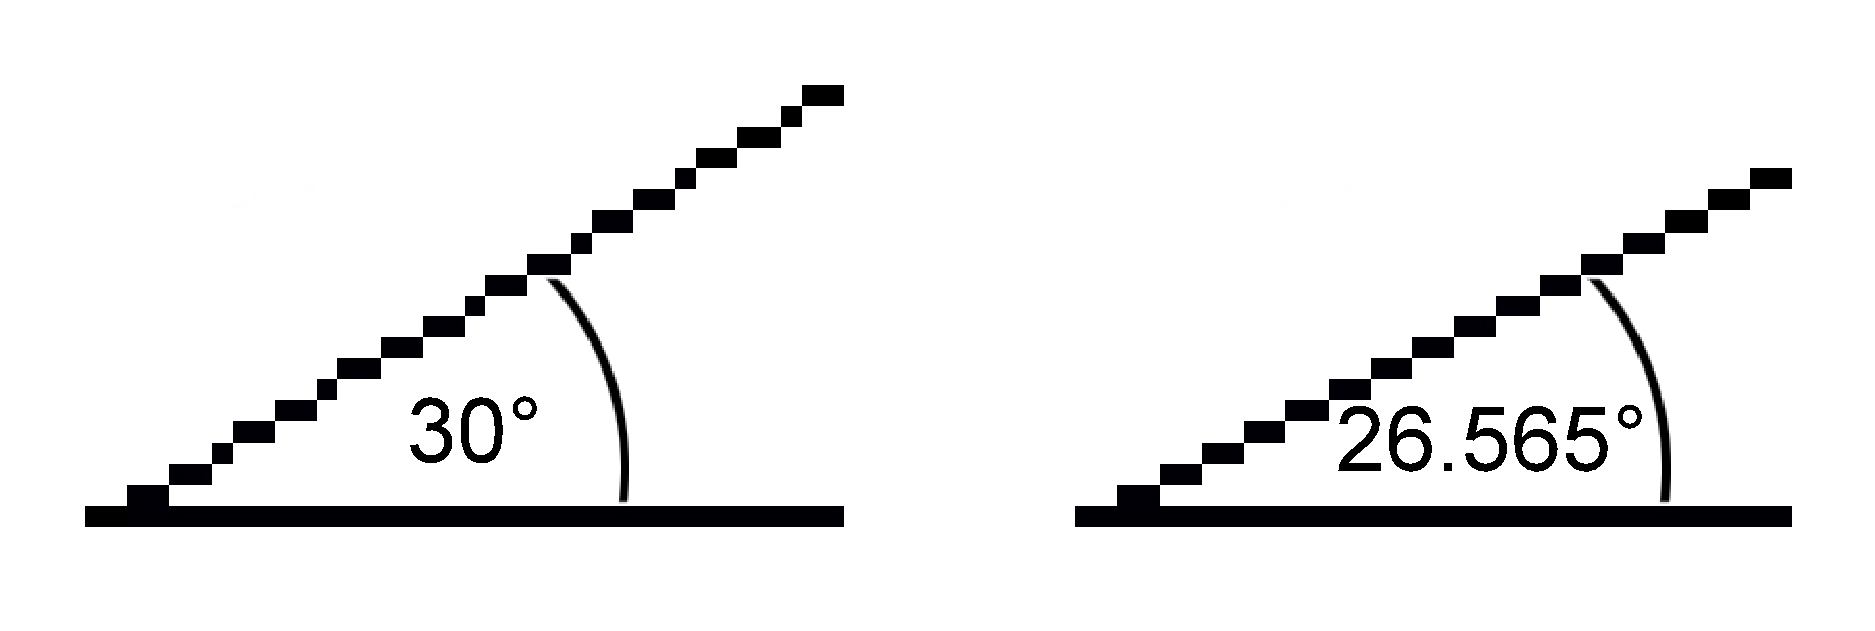
\includegraphics[width=0.7\textwidth]{thesis-angles}
	\caption{Isometric projection angle}
	\label{isoangle}
\end{figure}

\subsection{Example games, brief history}
The first game using isometric graphics was Zaxxon released by SEGA in 1982\cite{zaxxon} (see Figure \ref{zaxxon}). This new approach allowed display 3D scene without the need for hardware accelerated 3D rendering. Same graphic style was then used in many games, especially genres where the player overviews the scene from the top. In the 1990s, isometric graphics were common in games like Command\&Conquer or Transport Tycoon. These strategies often divided the map to regular tiles that limited the player actions but made collision detection and other mechanics very simple. This design outlived the slow hardware with no graphic acceleration and is still popular both among independent developers with limited resources and in environments where hardware acceleration is not granted\footnote{E.g. browser games discussed later.}.

\begin{figure}[htp]
	\centering
	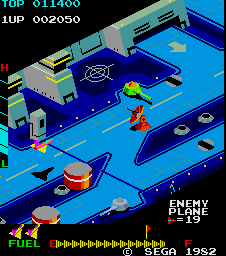
\includegraphics{zaxxon}
	\caption{Isometric graphics in original arcade version of Zaxxon\cite{zaxxon}}
	\label{zaxxon}
\end{figure}

\section{Web graphics, HTML5}
Web applications can on the client side rely only on the browser application and it's capabilities. No middleware directly accessing hardware is not guaranteed. Therefore the browser games\footnote{Games played on a web page displayed in the browser.} draw graphics to some element in the HTML page. Prior to the version 5 of standard HTML, the games almost exclusively used Flash\cite{} and required the client browser to have Flash Player plug-in\footnote{E.g. \href{https://get2.adobe.com/cz/flashplayer/}{Adobe Flash Player}} installed. With the broad adoption of HTML5, new options presented themselves. The two new elements to display graphics allow to stop making any assumptions about the client other than it supports HTML5. SVG element is very different as it displays given SVG. It can also be manipulated with JavaScript, but the approach is fundamentally different. Instead of redrawing the whole image or a part of screen, individual objects can be added, removed or manipulated. This makes e.g. animation of an object much more straight forward.

\subsection{Canvas, usage in games}
The canvas element is very similar to the canvas objects in other programming environments\footnote{E.g. classes System.Windows.Controls.Canvas in .NET framework\cite{net_canvas} or java.awt.Canvas in the Java platform\cite{java_canvas}}. It allows to directly draw to the canvas bitmap using JavaScript functions. Even though this approach is straight forward, some disadvantages arise when applied. Most noticeable is that when an object is being changed, everything that even partially covers it has to be re-drawn as well even if it stays unchanged. Also when drawing several objects that appear behind and in front of each other, these need to be carefully drawn in a correct order so the overlaps are correct.

\subsection{SVG}
SVG\footnote{Scalable Vector Graphics} is a markup language that uses XML to describe a vector image. Even though browsers used to support static SVG for a long time, not until HTML5 did they support dynamic in-line SVG\cite{}. This is now available with the eponymous element. Because rendering the markup language is much more complicated than simple pasting of the canvas bitmap on the screen, the browser support is delayed and also more sensitive to performance problems. Drawing to the canvas may take a lot of JavaScript execution time, but in the end the display of the element takes constant time. Creating large SVG will take similar time, but then rendering it on the screen will take browser another time. 
SVG needs different mindset compared to standard canvas. Elements are added to the DOM as if only standard HTML was used. These can be later modified, animated or removed. Also user interaction handling is easier, because event handlers can be hooked onto the elements representing the objects.

\chapter{Suggested solution}
\label{solution}
Can SVG be used to draw isometric game graphics instead of the standard canvas approach? If so, the SVG would make manipulation with specific objects in a drawn scene much easier.

\chapter{Used technologies}
\label{tech}
\section{Client}
The rendering engine is client-based and hence all technologies used in it are based around JavaScript.

\subsection{Browser support of used system JavaScript objects}
JSON, XmlHttpRequest

\subsection{Browser support of HTML5 SVG element}

\subsection{SVG manipulation JavaScript libraries}
There are several JavaScript libraries that provide abstract layer over SVG markup to.
What are the options, what did I pick and why

\subsection{General utility JavaScript libraries}
For each what does it do, why do I use it, source, license
\begin{itemize}
	\item require.js
	\item jQuery
\end{itemize}

\section{Server for testing purposes}
\subsection{RESTEasy}
jBoss REST library

\subsection{Jackson}
JSON serialization

\subsection{AppEngine API}
Google App Engine hosting

\chapter{Implementation}
\label{implementation}
Important part of the engine implementation is universality and therefore abstraction of all details of any specific game. Everything that would lead to these specifics is performed via calling handler functions on objects providing the specific game implementation.

\begin{figure}[htp]
	\centering
	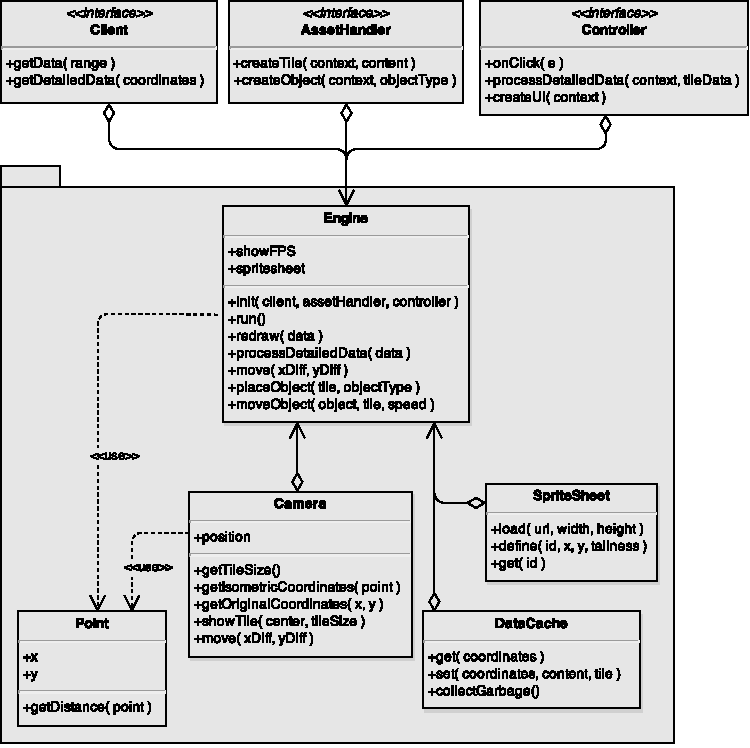
\includegraphics[width=\textwidth]{thesis-classdiagram}
	\caption{Diagram of the JavaScript modules}
	\label{classdiagram}
\end{figure}

\subsection{Viewport population and data fetching}
To populate the screen with tiles, data describing each of the tiles that will be displayed on the screen need to be obtained. That is performed via an asynchronous call to the client object that will in return call asynchronous callback on the engine after it obtains or creates the requested data. These data can be continuous array of tile content values or if the client determines that only a few tiles changed, only content and coordinates of these changed tiles can be returned. This will save data traffic when repeatedly requesting updates of the same area.

\subsection{Sprites}
The standard (citation needed) of making 2D games is to draw small images of objects and then compose the scene using these images. This way the object can be animated easily by replacing said image with next animation frame image. For performance reasons all these sprites are compiled to a single image called sprite-sheet. The graphic engine needs to be able to draw a sub-selection of the image. When working with HTML5 canvas element, JavaScript function context.drawImage(img,sx,sy,swidth,sheight,x,y,width,height) does exactly that. First set of of coordinates and dimensions determines which part of the source image will be drawn. When using SVG, no such a straightforward and convenient way is available. To display a section of an image, one needs to create a pattern from it and position it using a negative coordinates. The pattern must use objectBoundingBox units so it doesn't shrink the whole sprite-sheet in the target element. Then an SVG element (usually polygon) using this pattern can display desired selection of an image.
The limitation of this approach is that all elements using the same pattern must have synchronous animation, what usually doesn't look too organic in the result. On the other hand it nicely emulates the early 90s era of gaming.

\subsection{Object stacking and verticality}

\subsection{Features I did not implement with reasoning why not}

\chapter{Testing and measurement}
\label{testing}
\subsection{Performance on desktop and mobile devices}
Mobile devices were probably a long shot, even desktop browsers have vast differences in performance - in chrome everything runs nicely, Firefox is barely usable and Internet Explorer 11 is absolutely useless.

\chapter{Conclusion}
Evaluation of the results with emphasis on my contribution from the point of view of a wider context.
Future work, possible improvements - missing features, React.js to optimize the DOM manipulation.

\bibliographystyle{csplainnat} % sets plain bibliography style  
\bibliography{sources}     % BibTeX database file  

\appendix
\chapter{How to use my engine for your game}
The engine provides API makes the viewport manipulation very easy. The use of this API is demonstrated in the \href{https://github.com/vit-svoboda/svg-engine/tree/master/src/main/webapp/Scripts/game}{sample application}.

\section{Data feed}
Data describing what should be displayed are provided to the engine through an object passed as a first parameter of engine.init method. When engine needs data, methods getData or getDetailedData are called. This data can be obtained from a remote server using HTTP requests, stored in the client memory and passed directly or in any other way suitable for the given game.

\section{Asset management}
To give the game implementation power over what is displayed in place of data discussed earlier, everything displayed is translated using an object passed as a second parameter of the engine.init method. This translation is performed via methods createTile or createObject where the SVG drawing context is provided. Result is placed on the corresponding place in the viewport.

\section{UI handling and game logic}
The third object passed to the engine.init method is responsible for handling user interaction. method createUi is responsible for the standard UI displayed all the time, method processDetailedData is a handler for detailed tile data once it is obtained and method onClick is a handler for any tile or object clicked. Here most of the user interaction needs to be handled. Very little boundaries are given to other interaction implementation though.

\end{document} 